\documentclass[conference,compsoc]{IEEEtran}
\usepackage{datetime}
\usepackage{caption}
\usepackage{listings}
\usepackage{algorithm} 
\usepackage{algpseudocode} 
\lstdefinestyle{mystyle}{
    basicstyle=\small\sffamily,
	numbers=left,
	numberstyle=\tiny,
	frame=tb,
	breakatwhitespace=true,  
    	breaklines=true,
	columns=fullflexible,
	showstringspaces=false}
\usepackage[utf8]{inputenc}
\usepackage{menukeys}

% *** CITATION PACKAGES ***
%
\ifCLASSOPTIONcompsoc
  % IEEE Computer Society needs nocompress option
  % requires cite.sty v4.0 or later (November 2003)
  \usepackage[nocompress]{cite}
\else  
  % normal IEEE
  \usepackage{cite} 
\fi 
% cite.sty was written by Donald Arseneau
% V1.6 and later of IEEEtran pre-defines the format of the cite.sty package
% \cite{} output to follow that of the IEEE. Loading the cite package will
% result in citation numbers being automatically sorted and properly
% "compressed/ranged". e.g., [1], [9], [2], [7], [5], [6] without using
% cite.sty will become [1], [2], [5]--[7], [9] using cite.sty. cite.sty's
% \cite will automatically add leading space, if needed. Use cite.sty's
% noadjust option (cite.sty V3.8 and later) if you want to turn this off
% such as if a citation ever needs to be enclosed in parenthesis.
% cite.sty is already installed on most LaTeX systems. Be sure and use
% version 5.0 (2009-03-20) and later if using hyperref.sty.
% The latest version can be obtained at:
% http://www.ctan.org/pkg/cite
% The documentation is contained in the cite.sty file itself.
%
% Note that some packages require special options to format as the Computer
% Society requires. In particular, Computer Society  papers do not use
% compressed citation ranges as is done in typical IEEE papers
% (e.g., [1]-[4]). Instead, they list every citation separately in order
% (e.g., [1], [2], [3], [4]). To get the latter we need to load the cite
% package with the nocompress option which is supported by cite.sty v4.0
% and later.

% *** GRAPHICS RELATED PACKAGES ***
%
\ifCLASSINFOpdf
  % \usepackage[pdftex]{graphicx}
  % declare the path(s) where your graphic files are
  % \graphicspath{{../pdf/}{../jpeg/}}
  % and their extensions so you won't have to specify these with
  % every instance of \includegraphics
  % \DeclareGraphicsExtensions{.pdf,.jpeg,.png}
\else
  % or other class option (dvipsone, dvipdf, if not using dvips). graphicx
  % will default to the driver specified in the system graphics.cfg if no
  % driver is specified.
  % \usepackage[dvips]{graphicx}
  % declare the path(s) where your graphic files are
  % \graphicspath{{../eps/}}
  % and their extensions so you won't have to specify these with
  % every instance of \includegraphics
  % \DeclareGraphicsExtensions{.eps}
\fi
% graphicx was written by David Carlisle and Sebastian Rahtz. It is
% required if you want graphics, photos, etc. graphicx.sty is already
% installed on most LaTeX systems. The latest version and documentation
% can be obtained at: 
% http://www.ctan.org/pkg/graphicx
% Another good source of documentation is "Using Imported Graphics in
% LaTeX2e" by Keith Reckdahl which can be found at:
% http://www.ctan.org/pkg/epslatex
%
% latex, and pdflatex in dvi mode, support graphics in encapsulated
% postscript (.eps) format. pdflatex in pdf mode supports graphics
% in .pdf, .jpeg, .png and .mps (metapost) formats. Users should ensure
% that all non-photo figures use a vector format (.eps, .pdf, .mps) and
% not a bitmapped formats (.jpeg, .png). The IEEE frowns on bitmapped formats
% which can result in "jaggedy"/blurry rendering of lines and letters as
% well as large increases in file sizes.
%
% You can find documentation about the pdfTeX application at:
% http://www.tug.org/applications/pdftex


% *** MATH PACKAGES ***
%
\usepackage{amsmath}
% A popular package from the American Mathematical Society that provides
% many useful and powerful commands for dealing with mathematics.
%
% Note that the amsmath package sets \interdisplaylinepenalty to 10000
% thus preventing page breaks from occurring within multiline equations. Use:
%\interdisplaylinepenalty=2500
% after loading amsmath to restore such page breaks as IEEEtran.cls normally
% does. amsmath.sty is already installed on most LaTeX systems. The latest
% version and documentation can be obtained at:
% http://www.ctan.org/pkg/amsmath

% *** SPECIALIZED LIST PACKAGES ***
%
%\usepackage{algorithmic}
% algorithmic.sty was written by Peter Williams and Rogerio Brito.
% This package provides an algorithmic environment fo describing algorithms.
% You can use the algorithmic environment in-text or within a figure
% environment to provide for a floating algorithm. Do NOT use the algorithm
% floating environment provided by algorithm.sty (by the same authors) or
% algorithm2e.sty (by Christophe Fiorio) as the IEEE does not use dedicated
% algorithm float types and packages that provide these will not provide
% correct IEEE style captions. The latest version and documentation of
% algorithmic.sty can be obtained at:
% http://www.ctan.org/pkg/algorithms
% Also of interest may be the (relatively newer and more customizable)
% algorithmicx.sty package by Szasz Janos:
% http://www.ctan.org/pkg/algorithmicx


% *** ALIGNMENT PACKAGES ***
%
%\usepackage{array}
% Frank Mittelbach's and David Carlisle's array.sty patches and improves
% the standard LaTeX2e array and tabular environments to provide better
% appearance and additional user controls. As the default LaTeX2e table
% generation code is lacking to the point of almost being broken with
% respect to the quality of the end results, all users are strongly
% advised to use an enhanced (at the very least that provided by array.sty)
% set of table tools. array.sty is already installed on most systems. The
% latest version and documentation can be obtained at:
% http://www.ctan.org/pkg/array

% IEEEtran contains the IEEEeqnarray family of commands that can be used to
% generate multiline equations as well as matrices, tables, etc., of high
% quality.

% *** SUBFIGURE PACKAGES ***
%\ifCLASSOPTIONcompsoc
%  \usepackage[caption=false,font=footnotesize,labelfont=sf,textfont=sf]{subfig}
%\else
%  \usepackage[caption=false,font=footnotesize]{subfig}
%\fi
% subfig.sty, written by Steven Douglas Cochran, is the modern replacement
% for subfigure.sty, the latter of which is no longer maintained and is
% incompatible with some LaTeX packages including fixltx2e. However,
% subfig.sty requires and automatically loads Axel Sommerfeldt's caption.sty
% which will override IEEEtran.cls' handling of captions and this will result
% in non-IEEE style figure/table captions. To prevent this problem, be sure
% and invoke subfig.sty's "caption=false" package option (available since
% subfig.sty version 1.3, 2005/06/28) as this is will preserve IEEEtran.cls
% handling of captions.
% Note that the Computer Society format requires a sans serif font rather
% than the serif font used in traditional IEEE formatting and thus the need
% to invoke different subfig.sty package options depending on whether
% compsoc mode has been enabled.
%
% The latest version and documentation of subfig.sty can be obtained at:
% http://www.ctan.org/pkg/subfig

% *** FLOAT PACKAGES ***
%
%\usepackage{fixltx2e}
% fixltx2e, the successor to the earlier fix2col.sty, was written by
% Frank Mittelbach and David Carlisle. This package corrects a few problems
% in the LaTeX2e kernel, the most notable of which is that in current
% LaTeX2e releases, the ordering of single and double column floats is not
% guaranteed to be preserved. Thus, an unpatched LaTeX2e can allow a
% single column figure to be placed prior to an earlier double column
% figure.
% Be aware that LaTeX2e kernels dated 2015 and later have fixltx2e.sty's
% corrections already built into the system in which case a warning will
% be issued if an attempt is made to load fixltx2e.sty as it is no longer
% needed.
% The latest version and documentation can be found at:
% http://www.ctan.org/pkg/fixltx2e

%\usepackage{stfloats}
% stfloats.sty was written by Sigitas Tolusis. This package gives LaTeX2e
% the ability to do double column floats at the bottom of the page as well
% as the top. (e.g., "\begin{figure*}[!b]" is not normally possible in
% LaTeX2e). It also provides a command:
%\fnbelowfloat
% to enable the placement of footnotes below bottom floats (the standard
% LaTeX2e kernel puts them above bottom floats). This is an invasive package
% which rewrites many portions of the LaTeX2e float routines. It may not work
% with other packages that modify the LaTeX2e float routines. The latest
% version and documentation can be obtained at:
% http://www.ctan.org/pkg/stfloats
% Do not use the stfloats baselinefloat ability as the IEEE does not allow
% \baselineskip to stretch. Authors submitting work to the IEEE should note
% that the IEEE rarely uses double column equations and that authors should try
% to avoid such use. Do not be tempted to use the cuted.sty or midfloat.sty
% packages (also by Sigitas Tolusis) as the IEEE does not format its papers in
% such ways.
% Do not attempt to use stfloats with fixltx2e as they are incompatible.
% Instead, use Morten Hogholm'a dblfloatfix which combines the features
% of both fixltx2e and stfloats:
%
% \usepackage{dblfloatfix}
% The latest version can be found at:
% http://www.ctan.org/pkg/dblfloatfix

% *** PDF, URL AND HYPERLINK PACKAGES ***
%
%\usepackage{url}
% url.sty was written by Donald Arseneau. It provides better support for
% handling and breaking URLs. url.sty is already installed on most LaTeX
% systems. The latest version and documentation can be obtained at:
% http://www.ctan.org/pkg/url
% Basically, \url{my_url_here}.

% *** Do not adjust lengths that control margins, column widths, etc. ***
% *** Do not use packages that alter fonts (such as pslatex).         ***
% There should be no need to do such things with IEEEtran.cls V1.6 and later.
% (Unless specifically asked to do so by the journal or conference you plan
% to submit to, of course. )

% correct bad hyphenation here
\hyphenation{op-tical net-works semi-conduc-tor}
   
\usepackage{hyperref}
 
\begin{document}
\lstset{style=mystyle}
% 
% paper title
% Titles are generally capitalized except for words such as a, an, and, as,
% at, but, by, for, in, nor, of, on, or, the, to and up, which are usually
% not capitalized unless they are the first or last word of the title.
% Linebreaks \\ can be used within to get better formatting as desired.
% Do not put math or special symbols in the title.
\title{
	OrbitCalc - A simplified version of the solar system\\
{\small \today~-~\currenttime}}

 
% author names and affiliations
% use a multiple column layout for up to three different
% affiliations
\author{\IEEEauthorblockN{Henrik Klasen}
\IEEEauthorblockA{University of Luxembourg\\
Email: henrik.klasen.001@student.uni.lu}
\\
{\bf This report has been produced under the supervision of:}\\
\IEEEauthorblockN{Gabriel Garcia}
\IEEEauthorblockA{University of Luxembourg\\
Email: gabriel.garcia@uni.lu}%
}

% conference papers do not typically use \thanks and this command
% is locked out in conference mode. If really needed, such as for
% the acknowledgment of grants, issue a \IEEEoverridecommandlockouts
% after \documentclass

% for over three affiliations, or if they all won't fit within the width
% of the page (and note that there is less available width in this regard for
% compsoc conferences compared to traditional conferences), use this
% alternative format:
% 
%\author{\IEEEauthorblockN{Michael Shell\IEEEauthorrefmark{1},
%Homer Simpson\IEEEauthorrefmark{2},
%James Kirk\IEEEauthorrefmark{3}, 
%Montgomery Scott\IEEEauthorrefmark{3} and
%Eldon Tyrell\IEEEauthorrefmark{4}}
%\IEEEauthorblockA{\IEEEauthorrefmark{1}School of Electrical and Computer Engineering\\
%Georgia Institute of Technology,
%Atlanta, Georgia 30332--0250\\ Email: see http://www.michaelshell.org/contact.html}
%\IEEEauthorblockA{\IEEEauthorrefmark{2}Twentieth Century Fox, Springfield, USA\\
%Email: homer@thesimpsons.com}
%\IEEEauthorblockA{\IEEEauthorrefmark{3}Starfleet Academy, San Francisco, California 96678-2391\\
%Telephone: (800) 555--1212, Fax: (888) 555--1212}
%\IEEEauthorblockA{\IEEEauthorrefmark{4}Tyrell Inc., 123 Replicant Street, Los Angeles, California 90210--4321}}




% use for special paper notices
%\IEEEspecialpapernotice{(Invited Paper)}




% make the title area
\maketitle

%to remove for your report
%\footnote{}

% As a general rule, do not put math, special symbols or citations
% in the abstract
\begin{abstract}
With scientific endeavours becoming more cost intensive, there is a need to plan specific missions into minor details. In order of cutting cost to expensive missions, such as satellite launches and submarine drones, it is important to plan missions in high detail. Computational models can help to find the weak points of the mission, find extreme values of the devices and can help to set up a safe margin for the mission program. The development of one such computational model with a potential use case in space exploration is the topic of this Bachelor Semester Project. (5850)
\end{abstract}

% no keywords

% For peer review papers, you can put extra information on the cover
% page as needed:
% \ifCLASSOPTIONpeerreview
% \begin{center} \bfseries EDICS Category: 3-BBND \end{center}
% \fi
%
% For peerreview papers, this IEEEtran command inserts a page break and
% creates the second title. It will be ignored for other modes.
\IEEEpeerreviewmaketitle


\section{Introduction (190/400 words)}
% no \IEEEPARstart
The importance of simulations in the scientific world is rising. Not only do they provide a less cost-effective way of testing real life scenarios in a virtual twin of the current model of the world. It is cheaper for example, to test new aerodynamics concepts in a virtual environment, where modularity is easier, instead of using wind tunnels. For these wind tunnel tests, the components have to be produced, the wind tunnel has to be powered on and a large amount of energy has to be used for powering the wind tunnel. Not only is this way of testing resource exhaustive, but also not very environmentally friendly, as a big portion of these prototypes will end up as scrap and can partly not even be used any more.  \\
Simulations can provide near-real world environments, or at least emulate the behaviour of certain laws in physics. With these environments, we can reduce the amount of resources we use, by checking: is it the right way to achieve our goal? Can we optimize the behaviour of our test subject before producing it? 
\section{Project description ($\pm$ 10\% of total words) }
\subsection{Domains}
\subsubsection{Scientific}

\begin{itemize}
	\item \emph{Computational Modelling}: This domain is all about breaking down real life environments and behaviours into equations and algorithms for simulating the environment as good as possible with certain simplifications.
	\item \emph{Simulations}: Simulations are a computational approach to emulate real life behaviours of objects and environments on computers. They are used for example for optimizing the trajectories in space, simulating fluid dynamics or aerodynamics for optimizing the fuel efficiency of cars.
	\item \emph{Scientific Computing}: Scientific Computing is an interdisciplinary discipline bound to develop approaches for algorithms, models and software. These are used for simulating real world behaviour as close as possible. This means, that computational modelling and simulations are both a subset of scientific computing, which is the broader scientific topic. 
\end{itemize}
\subsubsection{Technical}
\begin{itemize}
	\item \emph{Unity}: A state of the art game engine for three dimensional and two dimensional games. With its powerful, built-in physics engine, it is able to also create realistic simulations, such as digital twinning, fluid simulations, as well as large field gravitational simulations, which is the goal in this project.
	\item \emph{Visual Studio}: A powerful code editor for all of the programming languages in the .NET Framework. This IDE has Unity integration, which simplifies the development of programs in Unity. 
	\item \emph{C\#}: An object-oriented, higher level programming language in the .NET framework, which was heavily influenced by C++ and Java. C\# is often used in cross-platform application development, game development and in Machine Learning applications.
\end{itemize}

\subsection{Targeted Deliverables}
\label{sec-deliverables}
\subsubsection{Scientific deliverables}
The scientific part of this Bachelor Semester Project is about modelling a suitable, simplified model of the solar system.\\
It will consist of three parts. The first part being about the fundamentals of computational modelling, which will take a look at the approach of breaking real world data down to a computable model. This model can be emulated by a computer program.\\
The second part is about modelling a model with some constraints and simplifications. This model will include the basics of orbital mechanics, as well as the fundamental concepts of Newtonian physics.\\ 
The scientific part will tackle the following scientific question: \emph{How can scientists model a simplified simulation of the solar system?} \\
To find a satisfying answer to this question, it is necessary to answer the related questions:
\begin{itemize}
	\item \emph{What is a computational model?}: This question aims on answering the most basic and fundamental question of this project. The results of this question are required to later on build and model the computational model.
	\item \emph{What environmental factors of the solar system have to be considered?}: This question aims on answering, \emph{how} the model will look like. This includes the examination of the utilized simplifications, methodologies and an analysis of the factors influencing the selection of specific approaches.
	\item \emph{How can the model be modelled? }: With this question, the goal is to find equations and algorithms that facilitate an accurate representation of the computational model. This part is meant to include all the orbital mechanics theory needed. 
\end{itemize}
As the goal is to find satisfying answers to the questions above, a state-of-the-art study will be conducted. 
Based on this study, the subsequent resources are used to address the scientific question:
\begin{itemize}
	\item \cite{PhysicsSimulationsLargeWorlds}: This publication is about the computational cost of large scale physics simulations. It will mainly be used in the section for the question "\emph{What environmental factors of the solar system have to be considered?}", as it is about modelling the computational model itself. 
	\item \cite{ComputationalModelling}: The main point in using this publication is to find out a way to properly model a computational model. It provides many examples for computational models for several different simulations, which might help when modelling the solar system later in the project.
	\item \cite{ScientificComputing}: This resource is about scientific computing. As its objective is to teach undergraduate students the fundamentals of scientific computing and numerical methods to model a simulation or whichever model needed, it is well suitable for this Bachelor Semester Project. It will be used for getting some insights on how scientific computing is used today and how it \emph{can} be used in this project.
\end{itemize}
With the use of these resources, the scientific part will focus on delivering the most useful and crucial information to develop a satisfying model of the solar system. The results of this part will later on be used in the technical part of this bachelor semester project, which is all about the implementation of a three dimensional solar system in Unity. In the last section of this part of the project, we will take a look at which factors cannot be simulated in the model developed and which parts could possibly be added in future extensions, but which exceed the scope of this project. \\
The overall goal of this deliverable is to ensure, that the reader can understand the design decisions in the technical part. The results of this section will be used as a fundamental basis of the technical deliverable and the implementation.

\subsubsection{Technical deliverables}
The technical part of this Bachelor Semester Project is about the implementation of the computational model developed in the scientific part. In fact, it is about the implementation of a virtual version of the solar system. \\
While the scientific part is more about the "\emph{What do we want to simulate?}", this part is more about the "\emph{How do we implement what we want to simulate?}". The goal with this deliverable is, to get to know how to implement scientific computing models in a given environment. \\
As for the technical deliverable, there is not as much literature such as official scientific papers or publications. The main source of information will be the scientific deliverable, e.g. for the equations describing the gravitational law. Next to that, the official Unity Documentation (linked in \cite{UnityDoc}) will be used for any further documentation regarding Unitys API. \\ 
The technical deliverable will provide some key features:
\begin{itemize}
	\item \emph{Gravity}: According to the Newtonian gravitational law. Further details will be in the scientific part of the report.
	\item \emph{Real scale}: The scale of the objects in the solar system will correspond to their actual scale in the real solar system. This will (hopefully) ensure a higher degree of realism and ease gravitational calculations, which are based on the distances.
	\item \emph{Realistic lighting}: As the sun is more or less the only high intensity light source in the solar system, the simulation will use a point light source which will shine light from the suns position. 
	\item \emph{User controllable Satellite}: This will help the user experience navigating a satellite in a three dimensional solar system with objects influencing the trajectory of the space probe.
\end{itemize}
The program will eventually include a Graphical User Interface, for which some parameters are needed. So far it is planned to include the parameters for two objects, mainly x-y-z position of the objects. It will be determined in this section, which data is going to be displayed in a light-weight interface, which provides the user enough information for controlling a satellite and camera (exact number of cameras to be determined in the report). For example, the data, currently planned to be displayed are: 
\begin{itemize}
	\item Velocity of user controlled camera: Measure how fast the user is going in the solar system
	\item Velocity of the satellite: Enable the user to calculate where the space probe will be when.
	\item Distance of the satellite to the sun: Locate the position of the satellite
	\item Coordinates of the satellite: Locate the satellite in a three-dimensional space
	\item Coordinates of the camera: Locate the user controlled camera in three-dimensional space
	\item Distance camera – Sun: Locate the camera on a relative basis in the solar system
	\item Labels of the planets: Locate the planets relative to the camera
	\item Planet orbit paths: Locate the orbits of the planets
	\item Satellite trajectory: Display the points, the satellite already passed to estimate the further trajectory
\end{itemize}
As the user will be able to control the camera, it will be required for this project, to map keys on the keyboard to certain movements, to enable the user to experience the virtual solar system. As of now, the keys are mapped as follows:
\begin{itemize}
	\item \keys{W} – Forwards movement relative to current rotation
	\item \keys{A} – Left movement relative to current rotation
	\item \keys{S} – Backwards movement relative to current rotation
	\item \keys{D} – Right movement relative to current rotation
	\item Left \keys{\shift} – Upwards movement relative to current rotation
	\item Left \keys{\ctrl} – Downwards movement relative to current rotation
	\item \keys{\arrowkeyleft} – Rotation Left (Z-Axis)
	\item \keys{\arrowkeyright} – Rotation Right (Z-Axis)
	\item \keys{\arrowkeyup} – Rotation Upwards (X-Axis)
	\item \keys{\arrowkeydown} – Rotation Downwards (X-Axis)
\end{itemize}
Also the  satellite will be controllable by the user, to ensure, that the user gets a better understanding of the complexity of navigating in a three-dimensional space under the influence of gravitational pull to other celestial bodies. 



% \subsection{Constraints}
% Provide all the constraints that were to be considered for the project.
% A constraint is a property that is agreed by you and your PAT to have been satisfied before starting the project.
% An example could be ``good level in Python programming''. 
% As a consequence the work done to satisfy the constraints cannot be presented as a deliverable of the BSP.

\section{Pre-requisites} 
Although all concepts used in the report will be explained in the report, it could be helpful, yet not mandatory, to understand the basic notions of the following topics. These are already known by the author before starting. 
\subsection{Scientific pre-requisites}
Before starting the Bachelor Semester Project, the student had some experience in orbital mechanics, which includes the basics of (gravitational) force vectors. \\
Next to that, the student had some experience in constructing mathematical and physical models with certain simplifications for computational ease.
\subsection{Technical pre-requisites}
As the technical deliverable is about the implementation of a basic solar system simulation in Unity, the student already knows how to work with Unitys' scaling, transformation and rotation system and their script application programming interfaces (APIs) in C\#. Also the basics of game and simulation development are known, as it was part of a small course in the Computer Science Summer Camp at Hochschule Trier.

\section{A computational model}
\label{sec-computational-model}
\subsection{Requirements (122/150 words)}
The requirement for this section is to explain with the given resources, the concept of a computational model. This includes the fundamental basics of how it came to be, as well as some insights on how they are usually developed and the scientific significance of them. For the explanation, it should be well understandable to any person, who understands the basics of computer science and is willing to read this bachelor semester project. This is to ensure that the author has well understood the topics of this section, as it will be the fundament of the upcoming sections and the technical part.\\
The results of this section will provide a step by step way to build a computational model of any kind. 
\subsection{Design (213/300 words)}
As there are only few resources providing a general overview on computational models, this section of the report will mainly be consisting of information found in \cite{ComputationalModelsIntroduction}.\\
Here, the following chapters will be used for finding results to the above scientific question:
\begin{itemize}
	\item Chapter 1: Problem Solving and Computing:
	\begin{itemize}
		\item 1.1: This is useful for finding the motivation for computational models. It explains the fundamental issue and already hints at, what is needed to develop such a model.
		\item 1.2: As it is also the goal of this report to find a step by step set of instructions for building a computational model, this section already provides a basic skeleton for this set of instructions. \\
		Regarding \ref{sec-computational-model}, the outline of steps will be used to construct a more detailed instruction set than given in the resource. 
		\item 1.3: This section will be used to find different ways to tackle different mathematical difficulties. It will help to set up a guideline for transforming the mathematical model with formulas into a computational model with algorithmic approaches. 
	\end{itemize}
	
\end{itemize}
Next to these information, the observations made during the first weeks of the semester in the development of the application will be used. This will not only provide meaningful results, but also show the real world development of the models.
\subsection{Production (514/400 words)}
A computational model is a mathematical and algorithmic construct describing real world behaviours in formulas and procedures. With this in mind, finding a computational model needs a few steps for developing the model. This process is called \emph{computational modelling} and involves a numerous count of observations to be made. \\
But all in all, the steps for setting up a computational model are quite general, as they are usually applied universally and then tuned to the individual model depending on the models complexity.
\subsubsection{Observation}
The basis of modelling a computational model emulating an environment is observation. This enables to understand the challenges of the environment and to understand the problem. With these in mind, it is also useful to observe certain behaviours of different objects and note them down as much as possible, as it will help in \ref{Mathematical-foundations} to find appropriate formulas to describe these behaviours. \\
Observation also enables to figure out factors with a minor impact, which might have to be left out for simplifying the model.
\subsubsection{Problem Description}
(acc. to \cite{ComputationalModelsIntroduction}, Ch. 1 Section 2)
The problem description is one of the most important steps of designing a computational model. By providing a detailed problem description, taking into account all the important aspects, the model is supposed to take into account. This helps to prioritize different observations for later considerations of which aspects are must-have and which ones are nice-to-have aspects. 
\subsubsection{Mathematical foundations to a model}
\label{Mathematical-foundations}
To further advance in the model, it is usually required to find formulas describing the observed behaviours of the model. \\
As most models are used in interdisciplinary research, such as physics, mathematics, chemistry and biology, it often implies using existing formulas of this discipline to find a well-working environment for the computational model. 
The formulas for this have to be as complete as possible, as it will be the basis for later on designing the algorithmic approaches in the next step (\ref{algorithmic-design}).
\subsubsection{Algorithmic design}
\label{algorithmic-design}
As the mathematical foundations are known from \ref{Mathematical-foundations}, this step is about the way of computing, i.e. the algorithm. As computers are usually resource and power limited, this step is very important. There are several factors to consider when designing an algorithm for a computational model, such as recursive and iterative approaches. \\
In general, iterative approaches are more favourable, as they usually have a lower space complexity while providing the same results as recursive methods or at least provide a similar degree of accuracy. \\
Designing the algorithm also implies to simplify the mathematical model where computationally needed to reduce the overall space and time complexity of the program. 
\subsubsection{Guideline for computational models}
With all of these steps in mind, it is possible to reduce them to easy questions as a guideline:
\label{Guide}
\begin{enumerate}
	\item What do we see? Which behaviour is observable?
	\item What do we want to do? What is the problem we try to solve and which properties does the model need?
	\item What formulas describe the behaviour of our model?
	\item How do we implement the model in terms of algorithmic approach?
\end{enumerate}
\subsection{Assessment (0/150 words)}
Provide any objective elements to assess that your deliverables do or do not satisfy the requirements described above. 


\section{Observation and Problem Definition}
\label{sec-modeling}
\subsection{Requirements (121/150 words)}
This section requires to execute steps 1-3 from \ref{Guide} in order of finding a computational model for the solar system. \\
It will be required to provide subsections for every step of the guide, similar to the sections of \ref{sec-computational-model}. These sections will contain the scientific findings and important points of the model. \\
Not only the scientific findings of this section will play a central role for this section, but also how they correlate to the steps found in \ref{Guide} and \emph{why} the results found, are important. \\
Based on this, the report will deliver the most crucial formulas of the model in this part, which are a necessity in \ref{sec-simplify}. Also this section will provide some general simplifications, such as negligible factors.
\subsection{Design (148/300 words)}
As section \ref{sec-computational-model} already contains a detailed look at computational models and computational modelling, this section will use the results of section \ref{sec-computational-model} and combine it with the formulas describing the solar system. This will then provide a mathematical/computational model of the solar system, for which the goal is to model algorithmic approaches to emulate the behaviour of the solar system. This modelling will be step by step according to the guideline found in \ref{sec-computational-model} and will illustrate the use of it on this example. \\
Additionally, next to the chapters used in the preceding section, this section will use the following sections of Chapter 1 of \cite{ComputationalModelsIntroduction}:
\begin{itemize}
	\item 1.4: As this section is a more detailed description of Computational modelling with more details on the development process, which are not needed in \ref{sec-computational-model}.
	\item 1.8: Section 1.8 provides a software development approach to the problem of computational models.
\end{itemize} 

\subsection{Production (400/400 words)}
With the plan of how to build a computational model, we can now start constructing the basic framework of the model for this project.
\subsubsection{Observable behaviour}
\label{observations}
Let us assume, we want to model the computational model for a three-dimensional space. Our solar system has 9 major objects, namely the sun and all planets. These objects have different behaviours each:\\
\emph{Sun}: The sun is the centre of our model, as it also is the centre of the solar system. This object, although in reality not static, stays in more or less the same place in the closed system (if we assume, that the solar system is a closed system). It is also very important to note, that the sun has a mass and a size.\\
\emph{Planets}: The planets revolve around a common centre of mass. Each orbit has an inclination $\alpha$, a major semi-axis $a$, a minor semi-axis $b$ and an eccentricity $\epsilon$. 
These orbits are determined by the attraction between all bodies. As the attraction between bodies is determined by mass $m$ and distance $r$, each planet has a mass, a size and a position. It is also observable, that the orbits do indeed change slightly over time, due to effects, such as orbital decay or certain constellations pulling the body more into a certain direction, thus impacting the orbit.\\
\emph{Satellite}: The satellite has a mass, a position and a velocity or acceleration. With these values, it is able to revolve around an other celestial object. All other celestial bodies are \emph{theoretically} also attracted to it, but since the mass of the satellite object is negligible, it can be left out without loss of generality.
\subsubsection{Problem definition}
\label{Problem-Def}
The model we want to develop will have to simulate the behaviour of the solar system. The main focus will have to be the satellite objects trajectory, such that it will suffice to simplify the behaviours of the remaining bodies in the solar system, such as the sun and planets. For the celestial bodies, simplifications which do not interfere with the accuracy have to be found. Furthermore it will be necessary to minimize heavy weight calculations to save on compute power to be able to run the simulation on a lower end machine. \\
Since it is easier to see odd behaviour, the simulation should also be displaying all calculated values in a three dimensional space, i.e. the movement should be visible.
\subsection{Assessment (0/150 words)}
Provide any objective elements to assess that your deliverables do or do not satisfy the requirements described above. 

\section{Mathematical approach and simplifications}
\label{sec-simplify}
\subsection{Requirements (107/150 words)}
This section will find formulas for the model described in \ref{Problem-Def}. It is required to explain every formula and to reason about the specific model. This will finally lead to the model completion and finalize design of the model to be implemented in \ref{sec-solar-system} and later sections. Furthermore will this section give details like scale of the model and assumptions to simplify the computations to ensure ease of computation. \\
It will be required to give the specific formulas and from these, to elaborate, why this formula is usable or not useful for this model. Then from results in \ref{observations} it will be necessary to deduct useful simplifications.
\subsection{Design (95/300 words)}
This section will take a look at the scale of the numbers used in the model developed in \ref{sec-modeling} and point out floating point and precision issues. Furthermore it will simplify some equations for ease of computation and also simplify some behaviour into constants.\\
Specifically, this section will use Chapter 1 of \cite{ComputationalModelsIntroduction}. Section 1.11 of this chapter is especially important, as it provides the necessary information regarding floating point precision, errors and accuracy. \\
To find issues in precision, the sections \ref{sec-computational-model} and \ref{sec-modeling} will be used to show the errors or complex calculation made.
\subsection{Production (600/400 words)}
To build a mathematical model of the environment we want to simulate, we need to look at the physics behind the environment. This involves finding formulas for the observed behaviour. To structure this in a similar way to the Observable behaviour section (\ref{observations}), we will take a look at the model object for object.
\subsubsection{Sun}
\hfill\newline
\label{Sun}
\emph{Theoretical aspects: }The centre of mass, or also known as barycentre, of the solar system is located close to the sun. This means that the sun also revolves around this barycentre, which changes over time. So in theory, the sun is not a fixed object in the solar system, which means, we would need to calculate the position every single moment.\\
\emph{Practical aspects: } Since vectorial computations are rather resource heavy and are quite complex to compute, we would like to simplify the model here. Let us therefore assume, that the position of the sun is fixed and it represents the centre of mass of the solar system. 
\subsubsection{Planets}\hfill\\
\label{Planets}
\emph{Theoretical aspects: } We know from \ref{observations}, that the planets revolve around the sun. Their orbits are approximately elliptic, though not fully elliptic, since the focus of the ellipsis is the barycentre of the system, which changes over time. This leads to small variations in the orbits. \\
\emph{Practical aspects: } As we already simplified the sun as a static object, we can further simplify this system by assuming, that the planetary orbits do not change over time. The variations in the orbits are related to the variations of the barycentre of the system. As we already cancelled these variations out in the simplification of the sun, we can also do this here. \\
Leaving out these small variations leads to a formula for orbits describing elliptical shapes with a certain angle $\alpha$.
$\begin{pmatrix}
	f_{x} + (a_{mj} \cdot cos(0.005 \cdot v) \\ 0\\
	f_{z} + (a_{min} \cdot sin(0.005 \cdot v)
\end{pmatrix} \cdot \begin{pmatrix}
	cos(\alpha) & -sin(\alpha) & 0 \\
	sin(\alpha) & cos(\alpha) & 0 \\
	0 & 0 & 1
\end{pmatrix} $

\subsubsection{Satellite}\hfill\\
\label{satellite}
\emph{Theoretical aspect: } As mentioned in \ref{observations}, the satellite has a mass $m_{sat}$. It is under the gravitational pull of all celestial bodies, such as sun and planets. This means, that it is a necessity to calculate the distance $r_{i}$ to all objects $O_{i}$.
Therefore let the celestial bodies $O_{i}$ be numbered from 1 to 10 and their masses be $m_{1}$ ... $m_{10}$ with distance $r_{1}$ ... $r_{10}$. Then the forces influencing the satellite would be:
$$ \vec{F} = \sum_{i=1}^{10}{\gamma \cdot \frac{m_{i} \cdot m_{sat}}{\vec{r_{i}}^{2}}} $$
This formula can be simplified, as $\gamma$ and $m_{sat}$ are all factors of every portion of the sum, so they can be seen as a constant factor. This means, that the simplified formula would be:
$$ \vec{F} = \gamma \cdot m_{sat} \cdot \sum_{i=1}^{10}{\frac{m_{i}}{\vec{r_{i}}^{2}}} $$
Since the goal is to find a formula for $\vec{v}$, we need to transform $\vec{F}$ to $\vec{a}$. We know that $\vec{a} = \frac{\vec{F}}{m_{sat}}$, which leads to:
$$ \vec{a} = \frac{\vec{F}}{m_{sat}} = \frac{\gamma \cdot m_{sat} \cdot \sum_{i=1}^{10}{\frac{m_{i}}{\vec{r_{i}}^{2}}}}{m_{sat}} = \gamma \cdot \sum_{i=1}^{10}{\frac{m_{i}}{\vec{r_{i}}^{2}}} $$
As we know, that acceleration $\vec{a}$ can be transformed to velocity $\vec{v}$ with the formula: 
$$ \vec{v}(t) = \vec{a} \cdot t^{2} + \vec{v_{0}} $$
\emph{Practical aspects: } Even though we want to minimize vectorial calculations, we cannot simulate the system without them. But to make it more efficient in terms of calculations, we have to see, where we can use iterative approaches. \\ 
Since our final formula for the vectorial velocity $\vec{v}$ has $\vec{a}$ inside, we can simply replace $\vec{a}$ by the formula for $\vec{a}$, such that we do not introduce a new variable for $\vec{a}$:
$$ \vec{v}(t) = (\gamma \cdot \sum_{i=1}^{10}{\frac{m_{i}}{\vec{r_{i}}^{2}}}) \cdot t^{2} + \vec{v_{0}} $$
For transforming this formula into a usable formula for the calculations later on, we need to replace $\vec{v_{0}}$ by something already known or calculated. Since we already know, that $\vec{v_{0}}$ is the starting velocity at a point $t_{0}$, we can reformulate the formula as:
$$ \vec{v_{n}}(t) = (\gamma \cdot \sum_{i=1}^{10}{\frac{m_{i}}{\vec{r_{i}}^{2}}}) \cdot (\Delta t)^{2} + \vec{v}_{n-1} $$
Where $ \Delta t$ is the time difference between the current and the previous calculation and $\vec{v}_{n-1}$ is the velocity calculated in the previous iterative step.
\subsection{Assessment (0/150 words)}
Provide any objective elements to assess that your deliverables do or do not satisfy the requirements described above. 

\section{The solar system}
\label{sec-solar-system}
\subsection{Requirements (105/150 words)}
In this section it is required to find explanations and pseudocode for the implementation of the solar system. This section will focus on the implementation of the "stable orbit script" (SOS) which is mainly responsible for the elliptical orbits in this system. It will also be required to look at the results from \ref{sec-modeling} and \ref{sec-simplify} as they provide the \emph{theoretical} aspects of this part. With these as the main points covered, it will also be necessary to take a look at the game objects and the addition of a script to such an object. This will include a detailed glimpse at Unitys scripting API. 
\subsection{Design (97/300 words)}
This section will mainly take results from \ref{Sun} and \ref{Planets} to find code snippets corresponding to the formulas. It will be strongly oriented along \cite{UnityDoc}, as it will be the environment, in which the simulation is going to be written in. \\
Not only is one requirement to find the pseudocode, but also to explain it, which will also be done using very simple syntax and clear explanations. This section represents Step 4 of the Guide from \ref{Guide}. \\ Since this guide is also derived from \cite{ComputationalModelsIntroduction}, it also represents the "Algorithmic design"-Step in Chapter 1.3 of the book. 
\subsection{Production (490/400 words)}
To start constructing the model, we defined in \ref{sec-simplify}, we need to find corresponding code for the behaviour described in \ref{sec-modeling} and the formulas found in \ref{Sun} and \ref{Planets}. \\
Let us therefore start with the Sun, as it is quite straight forward.
\subsubsection{Sun - Algorithmic approach and implementation}
As defined in \ref{Sun}, the sun should be modelled as a static object. This means, that we create a sphere in the simulation environment. As the sun is also a light source in the solar system, it is also a light source in the simulation. \\
Given, that the sun does not provide a constant light, but some variations in its intensity, we can model this as a particle effect with large particles to hide a part of the light emission in one direction. \\
As we also defined, that the sun has a mass, it gets the property of a rigid body, which simply adds a floating point number indicating the mass of the body. With the size of the star being the X-Y-Z dimensions, we can also check this point of the list of properties.
\subsubsection{Planet - Algorithmic approach and implementation} \hfill\\
Similar to the sun, a planet has a mass and a size. This implies, that the planet object also has the property of a rigid body object. 
As we know from \ref{Planets}, we want to simplify the orbits of the planets to an ellipsis with the sun in one of the foci. The formula for an ellipsis in three-dimensional space is also given in \ref{Planets} as:
$$\begin{pmatrix}
	f_{x} + (a_{mj} \cdot cos(0.005 \cdot v) \\ 0\\
	f_{z} + (a_{min} \cdot sin(0.005 \cdot v)
\end{pmatrix} \cdot \begin{pmatrix}
	cos(\alpha) & -sin(\alpha) & 0 \\
	sin(\alpha) & cos(\alpha) & 0 \\
	0 & 0 & 1
\end{pmatrix} $$
Given the fact, that calculating with matrices in programming languages such as C\#, is difficult, we will use the predefined data structure \textbf{Vector3D} from Unity. This data structure is of the type 3-tuple of type float, in the form (X-Coordinates | Y-Coordinates | Z-Coordinates). For manipulating the position of the planet object (a sphere), it is necessary to use the \textbf{transform.position(Vector3D)} method, which takes a Vector3D as input and adds it to the objects current position. This leads to a the position to change coordinates, which ultimately means, that the object changes coordinates (the definition of movement). \\
\textbf{The algorithm} \\
As already mentioned, Unity provides methods and classes for three dimensional space. For us, the following classes and methods are important:
\begin{itemize}
	\item Quaternion: The class of rotation matrices in Unity. 
	\begin{itemize}
		\item Euler: Takes an angle as input and outputs the corresponding rotation matrix for this angle. The angle is measured in degree
	\end{itemize}
	\item Vector3(D): The Vector3 or Vector3D class is the implementation of three-dimensional vectors in the Unity game engine. 
	\begin{itemize}
		\item \textbf{transform}: The transform attribute describes the position, rotation and the scale of the game object. To manipulate the position of the object, transform.position has to be called. Usually, the transform attribute is associated with the game object, on which the script applies, i.e. script applies on Mercury, then it takes the position of Mercury etc. 
	\end{itemize}
\end{itemize}
Translated to pseudocode, this would imply the following script.
\begin{algorithm}
	\caption{Planet orbits on ellipsis}
	\begin{algorithmic}[1]
		\Function{Frame update}{}
			\State $\alpha \leftarrow |\vec{v}|$ \Comment{Calculate how much the object moved}
			
			\State $x \leftarrow focus.x + (mj\_semiaxis \cdot \cos(alpha \cdot 0.005)$
			\State $y \leftarrow focus.y + (min\_semiaxis \cdot \sin(alpha \cdot 0.005)$
			\State $\vec{p} \leftarrow (x, 0, y)$ \Comment{Let p be the vector of position without rotation}
			\State $Q \leftarrow \alpha$ \Comment{Let Q be the rotation matrix}
			\State $position \leftarrow \vec{p} \cdot Q$
		\EndFunction
	\end{algorithmic}
\end{algorithm}

\subsection{Assessment (0/150 words)}

\section{Movement in three dimensions and time control}
\label{sec-movement-in-3D}
\subsection{Requirements (75/150 words)}
This section will be mostly about the camera, camera controller and the time controller scripts of the Unity project. It will focus on the coding aspects as well as some mathematical background from Linear Algebra, such as Vectors and point transformations. Since this section is not based on physics, it does not rely on results from \ref{sec-modeling} and \ref{sec-simplify}.\\
Instead, it will illustrate based on pseudocode the algorithmic approach of movement in three dimensional space. \\

\subsection{Design (85/300 words)}
This section mostly relies on \cite{UnityDoc} and Linear Algebra for coming up with formulas and code. Next to this, simple formulas from mechanical physics are used to show the relation between time and movement. This will result in a formula based on a time $t$ and a time factor $f$, such that all functions, such as $s(t), v(t), a(t)$ are dependent on $f \cdot t$. \\
To conclude, these formulas will then be translated into code, understandable by a computer using the Unity Programming Interface.
\subsection{Production (575/400 words)}
\subsubsection{Modelling the camera} \hfill \\
As the camera object is not part of the solar system, let us assume, that the forces present in the solar system do not affect the camera. This will let us simplify the camera movement to movement with a constant velocity $v$. As v is constant, we know from basic mechanical physics, that $$s(t) = v \cdot t$$ Since we want to move the object in three dimensions, we need to transform all variables, except the time $t$ into three-dimensional vectors. This implies, that in order of transforming the given formula for translation into a three-dimensional formula for translation, we will only have to use the vector $\vec{v}$, since t can be seen as a scalar. This means, that our formula is:
$$\vec{s}(t) = \vec{v} \cdot t + \vec{s_{0}}$$
where $s_{0}$ is the previous position of the camera.\\
Given, that we can also rotate the camera, we need to introduce a rotation matrix $Q$, which is given by the two rotation matrices around the x-axis and the y-axis.
Let $\Theta$ be the rotation around the x-axis and $\phi$ be the rotation around the y-axis.
$$ Q = \begin{pmatrix}
	1 & 0 & 0 \\
	0 & cos(\Theta) & -sin(\Theta)\\
	0 & sin(\Theta) & cos(\Theta)
\end{pmatrix}+\begin{pmatrix}
	cos(\phi) & 0 & sin(\phi) \\
	0 & 1 & 0 \\
	-sin(\phi) & 0 & cos(\phi)
\end{pmatrix} $$
To compute the position of the object after the rotation of the camera, it is necessary to multiply $\vec{v}$ with $Q$. This ensures, that the movement is relative to the rotation of the camera and not absolute, which means, that it would only move in the direction relative to the coordinate system (i.e. instead of moving forward on press of \keys{W} with a 90° rotation relative to origin, it would move sidewards relative to the camera).\\
This implies, that the final formula, with Q dependent on $\Theta$ and $\phi$, would be: $$
\vec{s}(t) = Q(\Theta, \phi) \cdot \vec{v} \cdot t$$
\label{CamMov}
To simplify the above formula in words: Instead of moving in an absolute coordinate system, relative to the origin, we define ourselves the camera as the origin of a new coordinate system, where x, y and z are always forwards/backwards, sidewards and up-/downwards. This means, that controlling the camera is a bit more natural, as it always going exactly where the user is expecting it to move.
\subsubsection{Time warp} \hfill\\
The idea behind time warp in this project is, to speed up the objects, while still having the same physics apply to them. This basically means, that any formula in dependence on $\Delta t$ (time-difference) will have to have a factor f to apply the time warp. \\
The main intention behind this is, to minimize the time for observation of some behaviour, such as planetary constellations, higher gravitational pull of the satellite in one direction and the planet orbits in general. \\
The only object, on which time warp does not apply is the main camera, as it does not have physical properties, because it is only a tool of visualization of the program.\\
To control the time warp factor, there is a script which controls every script dependent on time. For the planet orbit algorithm for example this would mean, that $\alpha = |\vec{v}| \cdot f$ instead of $\alpha = |\vec{v}|$. For the planet orbits, this implies, that the planet will move more distance in each frame, which eventually results in a higher velocity (in the model it stays the same, as all objects speed up by the same factor). In the end, this means, that all physical objects (i.e. celestial bodies and satellite) are affected by this, such that it does not introduce errors. \\
The keys for time warp are:
\begin{itemize}
	\item \keys{1} - Decrease time warp factor
	\item \keys{2} - Increase time warp factor
\end{itemize}
\subsection{Assessment (0/150 words)}
\section{Satellite and gravity}
\label{sec-satellite-gravity}
\subsection{Requirements (79/150 words)}
For this section it is required to provide the most important explanations on how Gravity and the satellite object are implemented in the editor. This includes (Pseudo-)Code snippets for the most important functions. Also section \ref{sec-movement-in-3D} has to be taken into account, as also the satellite object has to move in three dimensions. \\
Most importantly, this section takes results from \ref{sec-modeling} and \ref{sec-simplify} to provide an answer to the question: \emph{How is satellite movement implemented in this program?}
\subsection{Design (87/300 words)}
This section will focus on the technical aspects of the scientific findings from \ref{satellite}. Next to the algorithmic approach (as explained in \ref{algorithmic-design}), this section will take the time-warp feature into account, as well as satellite controls (prograde and retrograde). To conclude the technical part of the project, it will discuss, how the forces are calculated (with the formulas from \ref{satellite}) and how they apply to the object. The main resource for this section will be the previous sections and \cite{UnityDoc} for elaborating how the algorithm works.
\subsection{Production (672/400 words)}
As already discussed in \ref{satellite}, the satellite cannot be simplified to static orbits, as it is very much influenced by the bigger celestial bodies. With this in mind, there is a three step approach to coming up with the algorithm for the satellite object.
\begin{enumerate}
	\item Find all celestial bodies in the enclosed system, access the relevant data and plug it into the formula.
	\item Find a velocity $v_{0}$ and a gravitational constant $\gamma$, which enable the satellite to have a stable orbit (i.e. to not crash into the sun).
	\item Implement Prograde and Retrograde burning by scaling the vectors and time warp.
\end{enumerate}
To recall the relevant formula: 
$$ \vec{v_{n}}(t) = (\gamma \cdot \sum_{i=1}^{10}{\frac{m_{i}}{\vec{r_{i}}^{2}}}) \cdot (\Delta t)^{2} + \vec{v}_{n-1} $$
Given this formula, we can observe, that we require each celestial bodies position for calculating the distance $r_{i}$ and the celestial bodies mass $m_{i}$, as well as the satellites previous velocity vector $\vec{v}_{n-1}$.
\subsubsection{Determining celestial bodies, fetching data and finding constants} \hfill \\
Our model has ten celestial bodies (the sun, all planets and Pluto). Since we want to simplify our algorithm as much as possible, we can save all celestial bodies in a game object array, over which we can iterate. \\
As it is necessary to access this array every frame update, it is the most resource efficient, to initialize this game object array upon startup of the program. It is possible to do this, as the game objects do not change, but only the attributes get updated to different values. \\
Let us look at the important attribute classes for an example body. Given, that we want to calculate the distance from the satellite to the celestial body, we need the position.
\begin{figure}[!h]
	
	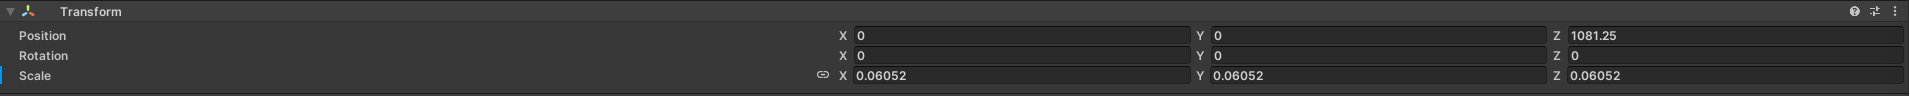
\includegraphics[width=\columnwidth]{Venus_vectors.png}
	\caption{Transform properties of an example celestial body.}
\end{figure}

The transform property is given in every game object and determines its position, scale and rotation. The algorithm will access this property to fetch the position and calculate the difference vector. The resulting vector is $\vec{r_{i}}$.
\begin{figure}[!h]
	
	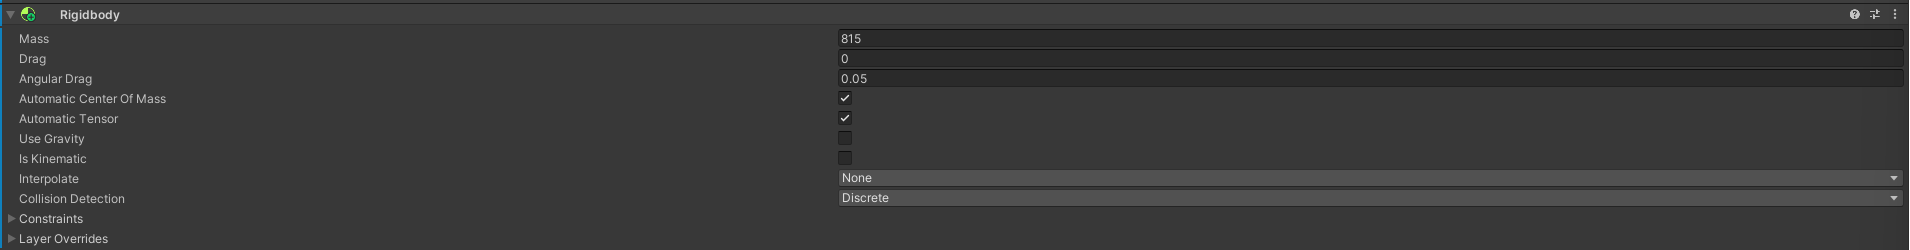
\includegraphics[width=\columnwidth]{Venus_rigid.png}
	\caption{Rigid body class determining mass.}
\end{figure}

The rigid body class has the public attribute mass. Instead of defining it on our own, which would not have been an issue, since it is just a floating point number, we access this attribute. In doing so, it might enable more future features if needed. The mass stored in the rigid body attribute will become the value $m_{i}$ for plugging into the formula. \\
Now, that all necessary data is fetched from the game objects after iterating over the array of celestial bodies, it is time to determine the constants. $\vec{v_{0}}$ and $\gamma$ have to be found. As the scale of the system is 1:1, but the mass-size proportion is not 1:1, $\gamma$ acts as a correcting factor. Instead of using the normal gravitational constant of $6.6743 \cdot 10^{-11}$, which is a very small number resulting in very small amount of force, the factor will be $66.743$. We simply multiply by $10^12$. The value of this was found in the trial and error method. Single precision floating point numbers are precise enough to represent this. \\
For $v_{0}$, we have the condition, that it enables the satellite object to have a stable orbit around the sun. If $v_{0}$ is too small, the satellite will have a collision course with the sun. If it is too large, it is going on an escape trajectory, eventually reaching a space, where the gravitational pull of the sun and all other celestial bodies become negligible.
\subsubsection{Prograde and retrograde orbit manipulation} \hfill\\
A spacecraft can alter its orbit by altering the vector of the resulting force. For prograde and retrograde orbit manipulation it is done by scaling the velocity vector by a scalar factor $p$. For this the following rules apply:
\begin{itemize}
	\item If $p < 1$: orbital velocity gets smaller, resulting in a lower orbit. This is a retrograde orbit manipulation.
	\item If $p > 1$: The orbital velocity gets higher, resulting in a higher orbit apoapsis. This is a prograde manipulation.
\end{itemize}
To apply this in the formula, we need to introduce p.
$$ \vec{v_{n}}(t) = p\cdot ((\gamma \cdot \sum_{i=1}^{10}{\frac{m_{i}}{\vec{r_{i}}^{2}}}) \cdot (\Delta t)^{2} + \vec{v}_{n-1}) $$
As we did not yet introduce time warp in this formula, it is necessary to change $\Delta t$ to $f\cdot \Delta t$.
$$ \vec{v_{n}}(t) = p\cdot((\gamma \cdot \sum_{i=1}^{10}{\frac{m_{i}}{\vec{r_{i}}^{2}}}) \cdot (f\cdot\Delta t)^{2} + \vec{v}_{n-1}) $$
\subsection{Assessment (0/150 words)}


\section*{Acknowledgment}
The author would like to thank his tutor for helping and guidance in the project and the Hochschule Trier for the Computer Science Summer Camps 2019 and 2021 which guided him to Computer Science and simulations.


\section{Conclusion}
The conclusion goes here.
\section{Plagiarism statement}

I declare that I am aware of the following facts:
\begin{itemize}
	\item As a student at the University of Luxembourg I must respect the rules of intellectual honesty, in particular not to resort to plagiarism, fraud or any other method that is illegal or contrary to scientific integrity.
	\item My report will be checked for plagiarism and if the plagiarism check is positive, an internal procedure will be started by my tutor. I am advised to request a pre-check by my tutor to avoid any issue.
	\item As declared in the assessment procedure of the University of Luxembourg, plagiarism is committed whenever the source of information used in an assignment, research report, paper or otherwise published/circulated piece of work is not properly acknowledged. In other words, plagiarism is the passing off as one’s own the words, ideas or work of another person, without attribution to the author. The omission of such proper acknowledgement amounts to claiming authorship for the work of another person. Plagiarism is committed regardless of the language of the original work used. Plagiarism can be deliberate or accidental.
	Instances of plagiarism include, but are not limited to:
	\begin{enumerate}
		\item Not putting quotation marks around a quote from another person’s work
		\item Pretending to paraphrase while in fact quoting
		\item Citing incorrectly or incompletely
		\item Failing to cite the source of a quoted or paraphrased work
		\item Copying/reproducing sections of another person’s work without acknowledging the source
		\item Paraphrasing another person’s work without acknowledging the source
		\item Having another person write/author a work for oneself and submitting/publishing it (with permission, with or without compensation) in one’s own name (‘ghost-writing’)
		\item Using another person’s unpublished work without attribution and permission (‘stealing’)
		\item Presenting a piece of work as one’s own that contains a high proportion of quoted/copied or paraphrased text (images, graphs, etc.), even if adequately referenced
	\end{enumerate}
	Auto- or self-plagiarism, that is the reproduction of (portions of a) text previously written by the author without citing that text, i.e. passing previously authored text as new, may be regarded as fraud if deemed sufficiently severe.
\end{itemize}

% An example of a floating figure using the graphicx package.
% Note that \label must occur AFTER (or within) \caption.
% For figures, \caption should occur after the \includegraphics.
% Note that IEEEtran v1.7 and later has special internal code that
% is designed to preserve the operation of \label within \caption
% even when the captionsoff option is in effect. However, because
% of issues like this, it may be the safest practice to put all your
% \label just after \caption rather than within \caption{}.
%
% Reminder: the "draftcls" or "draftclsnofoot", not "draft", class
% option should be used if it is desired that the figures are to be
% displayed while in draft mode.
%
%\begin{figure}[!t]
%\centering
%\includegraphics[width=2.5in]{myfigure}
% where an .eps filename suffix will be assumed under latex, 
% and a .pdf suffix will be assumed for pdflatex; or what has been declared
% via \DeclareGraphicsExtensions.
%\caption{Simulation results for the network.}
%\label{fig_sim}
%\end{figure}

% Note that the IEEE typically puts floats only at the top, even when this
% results in a large percentage of a column being occupied by floats.


% An example of a double column floating figure using two subfigures.
% (The subfig.sty package must be loaded for this to work.)
% The subfigure \label commands are set within each subfloat command,
% and the \label for the overall figure must come after \caption.
% \hfil is used as a separator to get equal spacing.
% Watch out that the combined width of all the subfigures on a 
% line do not exceed the text width or a line break will occur.
%
%\begin{figure*}[!t]
%\centering
%\subfloat[Case I]{\includegraphics[width=2.5in]{box}%
%\label{fig_first_case}}
%\hfil
%\subfloat[Case II]{\includegraphics[width=2.5in]{box}%
%\label{fig_second_case}}
%\caption{Simulation results for the network.}
%\label{fig_sim}
%\end{figure*}
%
% Note that often IEEE papers with subfigures do not employ subfigure
% captions (using the optional argument to \subfloat[]), but instead will
% reference/describe all of them (a), (b), etc., within the main caption.
% Be aware that for subfig.sty to generate the (a), (b), etc., subfigure
% labels, the optional argument to \subfloat must be present. If a
% subcaption is not desired, just leave its contents blank,
% e.g., \subfloat[].


% An example of a floating table. Note that, for IEEE style tables, the
% \caption command should come BEFORE the table and, given that table
% captions serve much like titles, are usually capitalized except for words
% such as a, an, and, as, at, but, by, for, in, nor, of, on, or, the, to
% and up, which are usually not capitalized unless they are the first or
% last word of the caption. Table text will default to \footnotesize as
% the IEEE normally uses this smaller font for tables.
% The \label must come after \caption as always.
%
%\begin{table}[!t]
%% increase table row spacing, adjust to taste
%\renewcommand{\arraystretch}{1.3}
% if using array.sty, it might be a good idea to tweak the value of
% \extrarowheight as needed to properly center the text within the cells
%\caption{An Example of a Table}
%\label{table_example}
%\centering
%% Some packages, such as MDW tools, offer better commands for making tables
%% than the plain LaTeX2e tabular which is used here.
%\begin{tabular}{|c||c|}
%\hline
%One & Two\\
%\hline
%Three & Four\\
%\hline
%\end{tabular}
%\end{table}


% Note that the IEEE does not put floats in the very first column
% - or typically anywhere on the first page for that matter. Also,
% in-text middle ("here") positioning is typically not used, but it
% is allowed and encouraged for Computer Society conferences (but
% not Computer Society journals). Most IEEE journals/conferences use
% top floats exclusively. 
% Note that, LaTeX2e, unlike IEEE journals/conferences, places
% footnotes above bottom floats. This can be corrected via the
% \fnbelowfloat command of the stfloats package.

% trigger a \newpage just before the given reference
% number - used to balance the columns on the last page
% adjust value as needed - may need to be readjusted if
% the document is modified later
%\IEEEtriggeratref{8}
% The "triggered" command can be changed if desired:
%\IEEEtriggercmd{\enlargethispage{-5in}}

% references section

% can use a bibliography generated by BibTeX as a .bbl file
% BibTeX documentation can be easily obtained at:
% http://mirror.ctan.org/biblio/bibtex/contrib/doc/
% The IEEEtran BibTeX style support page is at:
% http://www.michaelshell.org/tex/ieeetran/bibtex/
%\bibliographystyle{IEEEtran}
% argument is your BibTeX string definitions and bibliography database(s)
%\bibliography{IEEEabrv,../bib/paper}
%
% <OR> manually copy in the resultant .bbl file
% set second argument of \begin to the number of references
% (used to reserve space for the reference number labels box)
\begin{thebibliography}{1}
\bibitem[BiCS(2021)]{bics-bsp-report-template}
\newblock {BiCS Bachelor Semester Project Report Template}.
\newblock {https://github.com/nicolasguelfi/lu.uni.course.bics.global}
\newblock {University of Luxembourg, BiCS - Bachelor in Computer Science (2021).}

\bibitem[BiCS(2021)] {bics-bsp-reference-document}
{Bachelor in Computer Science}:
\newblock {BiCS Semester Projects Reference Document}.
\newblock Technical report, University of Luxembourg (2021)

\bibitem[Armstrong and Green(2017)]{armstrong2017guidelinesforscience}
J~Scott Armstrong and Kesten~C Green.
\newblock Guidelines for science: Evidence and checklists.
\newblock \emph{Scholarly Commons}, pages 1--24, 2017.
\newblock {https://repository.upenn.edu/marketing\_papers/181/}

	\bibitem[BiCS(2021)]{bics-bsp-report-template}
	\newblock {BiCS Bachelor Semester Project Report Template}.
	\newblock {https://github.com/nicolasguelfi/lu.uni.course.bics.global}
	\newblock {University of Luxembourg, BiCS - Bachelor in Computer Science (2021).}
	
	\bibitem[BiCS(2021)] {bics-bsp-reference-document}
	{Bachelor in Computer Science}:
	\newblock {BiCS Semester Projects Reference Document}.
	\newblock Technical report, University of Luxembourg (2021)
	
	\bibitem[Armstrong and Green(2017)]{armstrong2017guidelinesforscience}
	J~Scott Armstrong and Kesten~C Green.
	\newblock Guidelines for science: Evidence and checklists.
	\newblock \emph{Scholarly Commons}, pages 1--24, 2017.
	\newblock {https://repository.upenn.edu/marketing\_papers/181/}
	
	\bibitem[KaufmannFranzinMenegaisPozzer]{PhysicsSimulationsLargeWorlds}
	Lorenzo Schwertner Kaufmann, Flavio Paulus Franzin, Roberto Menegais, Cesar Tadeu Pozzer.
	\newblock Accurate Real-Time Physics Simulation for Large Worlds.
	\newblock \emph{Universidade Federal de Santa Maria, Santa Maria, Brazil}, 2021.
	
	\bibitem[MurinKompisKutis]{ComputationalModelling}
	Justin Murin, Vladimir Kompis, Vladimir Kutis.
	\newblock Computational Modelling and Advanced Simulations. \\
	\newblock \emph{Springer}, 978-94-007-0317-9-1, 2011.
	
	\bibitem[HeisterRebholz]{ScientificComputing}
	Timo Heister, Leo G. Rebholz.
	\newblock Scientific Computing for Scientists and Engineers.
	\newblock \emph{De Gruyter}, 2023.
	
	\bibitem[Garrido]{ComputationalModelsIntroduction}
	Jose M. Garrido
	\newblock Introduction to Computational Models with Python
	\newblock \emph{Chapman and Hall/CRC}, 2016.
	
	\bibitem[Unity]{UnityDoc}
	\newblock \href{https://docs.unity3d.com/Manual/index.html}{https://docs.unity3d.com/Manual/index.html}

\end{thebibliography}
\newpage 
\section{Appendix}
All images and additional material go there.

\subsection{Source Code}

\begin{lstlisting}

\end{lstlisting}
% that's all folks

\end{document}


